\chapter{Background}
\label{theory_of_quantum_information}
\section{ Quantum Computing}

 In this chapter, the author will provide fundamental knowledge about quantum computing, including the concepts of quantum bits, quantum gates, quantum circuit and quantum compilation.

\subsection{Quantum Bit}

 A classical bit has two different states, which are 0 and 1.   Instead, those of a quantum bit (or \textbf{qubit} in short) are $|0\rangle$ and $|1\rangle$, each of which can be described as a vector.  
 $$|0\rangle = \left[
\begin{array}{c}
1 \\
0 \\
\end{array}
\right]$$
 $$|1\rangle = \left[
\begin{array}{c}
0 \\
1 \\
\end{array}
\right]$$

The state of a single 	qubit $|\psi\rangle$ can be described as follows.
$$ |\psi\rangle = \alpha |0\rangle + \beta |1\rangle \,(\alpha, \beta \in \mathbb{C}, |\alpha|^2+|\beta|^2=1)$$
 After the operation called measurement, the quantum state would be collapsed into either 0 or 1.  The measurement probability of 0 is $|\alpha|^2$ and that of 1 is $|\beta|^2$. In other words, a single qubit can take both states probabilistically at the same time.  For instance, a qubit can be 
 
\begin{equation}
	|\psi\rangle = \frac{1}{\sqrt{2}}|0\rangle + \frac{1}{\sqrt{2}}|1\rangle \tag{1}
\end{equation}

 which can be 50\% 0 and 50\% 1.
 
 \subsection{Bloch sphere}
 	Because $|\alpha|^2 + |\beta|^2 = 1$, the notation of a single qubit state can be represented like this.
	
\begin{equation}
	|\psi\rangle = e^{i\gamma} (\cos{\frac{\theta}{2}} + e^{i\phi} \sin{\frac{\theta}{2}}) (\gamma, \phi, \theta \in \mathbb{R})
\end{equation} 

	Because $e^{i\gamma}$ is just a global state, it can be ignored and the same state can be rewritten like this.
	
\begin{equation}
	 |\psi\rangle =  \cos{\frac{\theta}{2}} + e^{i\phi} \sin{\frac{\theta}{2}} (\phi, \theta \in \mathbb{C})
\end{equation} 

	Because the equation above has two parameters,  any pure single qubit state can be considered as a point on the surface and its geometric representation is called \textbf{Bloch sphere}.
	
\begin{figure}[ht]
\centering
\tikz{
  \tikzstyle{st}=[lightgray, fill, fill opacity=0.2];
  \coordinate(o)at(0,0);
  \draw(o)circle(2cm);
  \draw[fill](o)circle(1.5pt);%origin
  \draw[st](o)--(56.7:0.4)arc(56.7:90.:0.4)--cycle;%theta angle
  \draw(0.18,0.6)node{$\theta$};
  \draw[st](o)--(-135.7:0.4)arc(-135.7:-33.2:0.4)--cycle;%varphi angle
  \draw(0.14,-0.58)node{$\varphi$};
  \draw[->](o)--(-0.81,-0.79) node[above left]{\ $x$};%x
  \draw[->](o)--(2,0)node[right]{$y$};%y
  \draw[->](o)--(0,2)node[below right]{$z$}node[above]{\ $\ket{0}$};%z |0>
  \draw[rotate around={0.:(0.,0.)},dashed](0,0)ellipse(2cm and 0.9cm);%ellipse
  \draw[thick,->](o)--(0.70,1.07)node[above]{\ $\ket{\psi}$};%state vector
  \draw[densely dotted,->](o)--(0,-2)node[below]{\ $\ket{1}$};%-z |1>
  \draw[dotted](o)--(0.7,-0.46)--(0.7,1);%triangle
  }
 \caption{Bloch Sphere}
 \end{figure}
	
 \subsection{Multi-Qubit State}
  The quantum state for multi-qubits is a \textbf{tensor product} of a state vector of each qubit.  The general notation of two qubit state is
   $$ |\psi\rangle = (\alpha |0\rangle + \beta |1\rangle) \otimes  (\gamma |0\rangle + \delta |1\rangle) $$
   
\begin{equation}
    = \alpha \gamma |00\rangle + \alpha \delta |01\rangle + \beta \gamma |10\rangle + \beta \delta |11\rangle 
\end{equation}
  $$(\alpha, \beta, \gamma, \delta \in \mathbb{C}, |\alpha|^2+|\beta|^2+|\gamma|^2+|\delta|^2=1)$$
  
  For example, the state $|00\rangle$ is equal to 
  
\begin{equation}
 \left[
\begin{array}{c}
1 \\
0 \\
\end{array}
\right]
\otimes
 \left[
\begin{array}{c}
1 \\
0 \\
\end{array}
\right]
= \left[
\begin{array}{c}
1 \\
0 \\
0 \\
0 \\
\end{array}
\right]
\end{equation}

 However, some quantum states such as
 
 \begin{equation}
 	|\psi\rangle = \frac{1}{\sqrt{2}}|00\rangle + \frac{1}{\sqrt{2}}|11\rangle
 \end{equation}
 
 cannot be decomposed into quantum state of each qubit.  These special quantum states are called \textbf{entangled} states.

\subsection{Quantum Gates}

 In this section, the author will talk about "logical gates" for quantum computers, which are called \textbf{quantum gates}.
 
\subsubsection{I gate}

I gate is equal to the 2x2 identity matrix, which is 

\begin{equation}
 I = \begin{bmatrix}
1 & 0 \\
0 & 1 \\
\end{bmatrix}
\end{equation}

For example,

\begin{equation}
 I|0\rangle = \begin{bmatrix}
1 & 0 \\
0 & 1 \\
\end{bmatrix} 
\left[
\begin{array}{c}
1 \\
0 \\
\end{array}
\right]
= \left[
\begin{array}{c}
1 \\
0 \\
\end{array}
\right]
= |0\rangle
\end{equation}

\begin{equation}
X|1\rangle = \begin{bmatrix}
1 & 0 \\
0 & 1 \\
\end{bmatrix} 
\left[
\begin{array}{c}
0 \\
1  \\
\end{array}
\right]
= \left[
\begin{array}{c}
0 \\
1 \\
\end{array}
\right]
= |1\rangle
\end{equation}


\subsubsection{X gate}

X gate flips the logical value of a qubit.

\begin{equation}
X = \begin{bmatrix}
0 & 1 \\
1 & 0 \\
\end{bmatrix}
\end{equation}

For example,
\begin{equation}
X|0\rangle = \begin{bmatrix}
0 & 1 \\
1 & 0 \\
\end{bmatrix} 
\left[
\begin{array}{c}
1 \\
0 \\
\end{array}
\right]
= \left[
\begin{array}{c}
0 \\
1 \\
\end{array}
\right]
= |1\rangle
\end{equation}

\begin{equation}
 X|1\rangle = \begin{bmatrix}
0 & 1 \\
1 & 0 \\
\end{bmatrix} 
\left[
\begin{array}{c}
0 \\
1  \\
\end{array}
\right]
= \left[
\begin{array}{c}
1 \\
0 \\
\end{array}
\right]
= |0\rangle
\end{equation}

\subsubsection{Y gate}

Y gate flips the logical value of a qubit and add an imaginary number.

\begin{equation}
 Y = \begin{bmatrix}
0 & -i \\
i & 0 \\
\end{bmatrix}
\end{equation}

For example,
\begin{equation}
Y|0\rangle = \begin{bmatrix}
0 & -i \\
i & 0 \\
\end{bmatrix} 
\left[
\begin{array}{c}
1 \\
0 \\
\end{array}
\right]
= \left[
\begin{array}{c}
0 \\
i \\
\end{array}
\right]
= i|1\rangle
\end{equation}

\begin{equation}
Y|1\rangle = \begin{bmatrix}
0 & -i \\
i & 0 \\
\end{bmatrix} 
\left[
\begin{array}{c}
0 \\
1  \\
\end{array}
\right]
= \left[
\begin{array}{c}
-i \\
0 \\
\end{array}
\right]
= -i|0\rangle
\end{equation}

\subsubsection{Z gate}

Z gate flips the phase of $ |1\rangle$

\begin{equation}
 Z = \begin{bmatrix}
1 & 0 \\
0 & -1 \\
\end{bmatrix}
\end{equation}

For example,
\begin{equation}
 Z|0\rangle = \begin{bmatrix}
1 & 0 \\
0 & -1 \\
\end{bmatrix} 
\left[
\begin{array}{c}
1 \\
0 \\
\end{array}
\right]
= \left[
\begin{array}{c}
1 \\
0 \\
\end{array}
\right]
= |0\rangle
\end{equation}

\begin{equation}
Z|1\rangle = \begin{bmatrix}
1 & 0 \\
0 & -1 \\
\end{bmatrix} 
\left[
\begin{array}{c}
0 \\
1  \\
\end{array}
\right]
= \left[
\begin{array}{c}
0 \\
-1 \\
\end{array}
\right]
= -|1\rangle
\end{equation}

\subsubsection{H gate}

H gate creates superposition.
\begin{equation}
 H = \frac{1}{\sqrt{2}}\begin{bmatrix}
1 & 1\\
1 & -1 \\
\end{bmatrix}
\end{equation}

For example,
\begin{equation}
H|0\rangle = \frac{1}{\sqrt{2}}\begin{bmatrix}
1 & 1\\
1 & -1 \\
\end{bmatrix}\left[
\begin{array}{c}
1 \\
0 \\
\end{array}
\right]
= \frac{1}{\sqrt{2}} \left[
\begin{array}{c}
1 \\
1 \\
\end{array}
\right]
= \frac{1}{\sqrt{2}} (|0\rangle + |1\rangle)
\end{equation}

\begin{equation}
H|1\rangle = \begin{bmatrix}
1 & 1\\
1 & -1 \\
\end{bmatrix} 
\left[
\begin{array}{c}
0 \\
1  \\
\end{array}
\right]
= \frac{1}{\sqrt{2}} \left[
\begin{array}{c}
1 \\
-1 \\
\end{array}
\right]
=\frac{1}{\sqrt{2}} (|0\rangle - |1\rangle)
\end{equation}

\subsubsection{Rx gate}
 An Rx gate rotate the given quantum circuit on the x-axis of the Bloch sphere.
 
 \begin{equation}
  Rx(\theta) = \begin{bmatrix}
\cos{\frac{\theta}{2}} & -i\sin{\frac{\theta}{2}} \\
 -i\sin{\frac{\theta}{2}} & \cos{\frac{\theta}{2}}  \\
\end{bmatrix}
\end{equation}
 
 For example,
 \begin{equation}
 Rx(\theta)|0\rangle = \begin{bmatrix}
\cos{\frac{\theta}{2}} & -i\sin{\frac{\theta}{2}} \\
 -i\sin{\frac{\theta}{2}} & \cos{\frac{\theta}{2}}  \\
\end{bmatrix}\left[
\begin{array}{c}
1 \\
0 \\
\end{array}
\right]
=  \left[
\begin{array}{c}
\cos{\frac{\theta}{2}} \\
-i\sin{\frac{\theta}{2}} \\
\end{array}
\right]
= \cos{\frac{\theta}{2}}|0\rangle -i \sin{\frac{\theta}{2}} |1\rangle
\end{equation}

\begin{equation}
Rx(\theta)|1\rangle = \begin{bmatrix}
\cos{\frac{\theta}{2}} & -i\sin{\frac{\theta}{2}} \\
 -i\sin{\frac{\theta}{2}} & \cos{\frac{\theta}{2}}  \\
\end{bmatrix}\left[
\begin{array}{c}
0 \\
1 \\
\end{array}
\right]
=  \left[
\begin{array}{c}
 -i\sin{\frac{\theta}{2}} \\
\cos{\frac{\theta}{2}}\\
\end{array}
\right]
=-i \sin{\frac{\theta}{2}}|0\rangle + \cos{\frac{\theta}{2}}|1\rangle
\end{equation}

\subsubsection{Ry gate}

 An Ry gate rotate the given quantum circuit on the y-axis of the Bloch sphere.
 
 \begin{equation}
 Ry(\theta) = \begin{bmatrix}
\cos{\frac{\theta}{2}} & -i\sin{\frac{\theta}{2}} \\
 -i\sin{\frac{\theta}{2}} & \cos{\frac{\theta}{2}}  \\
\end{bmatrix}
\end{equation}

\subsubsection{CNOT gate}

A CNOT gate involves two qubits, one is called \textbf{controlled qubit} and the other is called \textbf{target qubit}.  If the controlled qubit is 1, the bit value of the target qubit is flipped.

\begin{equation}
CNOT = \begin{bmatrix}
1 & 0 & 0 & 0 \\
0 & 1 & 0 & 0 \\
0 & 0 & 0 & 1 \\
0 & 0 & 1 & 0 \\
\end{bmatrix}
\end{equation}

\begin{equation}
CNOT_{0,1}|10\rangle = 
\begin{bmatrix}
1 & 0 & 0 & 0 \\
0 & 1 & 0 & 0 \\
0 & 0 & 0 & 1 \\
0 & 0 & 1 & 0 \\
\end{bmatrix}
 \left[
\begin{array}{c}
0 \\
0 \\
1 \\
0 \\
\end{array}
\right]
=  \left[
\begin{array}{c}
0 \\
0 \\
0 \\
1 \\
\end{array}
\right] 
= |11\rangle 
\end{equation}

\begin{equation}
CNOT_{0,1}|11\rangle = 
\begin{bmatrix}
1 & 0 & 0 & 0 \\
0 & 1 & 0 & 0 \\
0 & 0 & 0 & 1 \\
0 & 0 & 1 & 0 \\
\end{bmatrix}
 \left[
\begin{array}{c}
0 \\
0 \\
0 \\
1 \\
\end{array}
\right]
=  \left[
\begin{array}{c}
0 \\
0 \\
1 \\
0 \\
\end{array}
\right] 
= |10\rangle 
\end{equation}

\subsubsection{Quantum gate for multi-qubit system}

Just like quantum state of a multi-qubit system, the composited quantum gates is the tensor product of quantum gates that are applied on each qubit.  \\For example, 
\begin{equation}
X_0 \otimes X_1 = 
\begin{bmatrix}
0 & 1 \\
1 & 0 \\
\end{bmatrix}
\otimes
 \begin{bmatrix}
0 & 1 \\
1 & 0 \\
\end{bmatrix}
=  \begin{bmatrix}
0 & 0 & 0 & 1 \\
0 & 0 & 1 & 0 \\
0 & 1 & 0 & 0 \\
1 & 0 & 0 & 0 \\
\end{bmatrix}
\end{equation}

Therefore, 
\begin{equation}
 X_0X_1 |00\rangle = 
\begin{bmatrix}
0 & 0 & 0 & 1 \\
0 & 0 & 1 & 0 \\
0 & 1 & 0 & 0 \\
1 & 0 & 0 & 0 \\
\end{bmatrix}
\left[
\begin{array}{c}
1 \\
0 \\
0 \\
0 \\
\end{array}
\right] 
= \left[
\begin{array}{c}
0 \\
0 \\
0 \\
1 \\
\end{array}
\right] 
= |11\rangle
\end{equation}

\begin{equation}
 X_1 |00\rangle = 
I_0X_1 = 
\begin{bmatrix}
1 & 0 \\
0 & 1 \\
\end{bmatrix}
\otimes
\begin{bmatrix}
0 & 1 \\
1 & 0 \\
\end{bmatrix}
= \begin{bmatrix}
0 & 1 & 0 & 0 \\
1 & 0 & 0 & 0 \\
0 & 0 & 0 & 1 \\
0 & 0 & 1 & 0 \\
\end{bmatrix}
\end{equation}

\begin{equation}
I_0 X_1 |00\rangle
=  \begin{bmatrix}
0 & 1 & 0 & 0 \\
1 & 0 & 0 & 0 \\
0 & 0 & 0 & 1 \\
0 & 0 & 1 & 0 \\
\end{bmatrix}
\left[
\begin{array}{c}
1 \\
0 \\
0 \\
0 \\
\end{array}
\right] 
= \left[
\begin{array}{c}
0 \\
1 \\
0 \\
0 \\
\end{array}
\right] 
= |01\rangle
\end{equation}

\subsubsection{Measurement}

If a person measure a single qubit, he would get either 0 or 1 and that operation completely destroys the quantum state.  It will return 00, 01, 10, 11 in the case of two qubits.

\subsection{Quantum Circuit}

Here is the example of a quantum circuit.

$$
\begin{quantikz}
\ket{0} & \gate{H} & \qw & \ctrl{1} & \gate{X} & \gate{Y} &\meter{} && \\
\ket{0} & \gate{H} & \qw & \targ{} & \ctrl{1} & \gate{H} & \meter{}\\
\ket{0} & \gate{H} & \qw & \gate{X} & \targ{} & \qw & \meter{} \
\end{quantikz}
$$

Each horizontal line represents each qubit and the square boxes that contain alphabets mean single quantum gates.  The sign which involves a vertical line means a CNOT gate, and the box on the most right side indicates measurement. 

\subsection{Bell state}

In the chapter 1.3, the author mentions about a special type of quantum states called entangled states, and there are four specific quantum states called "Bell state", which are

\begin{equation}
 |\Phi^+\rangle = \frac{|00\rangle + |11\rangle}{\sqrt{2}}
 \end{equation}
 
 \begin{equation}
|\Phi^-\rangle = \frac{|00\rangle - |11\rangle}{\sqrt{2}}
\end{equation}

\begin{equation}
|\Psi^+\rangle = \frac{|01\rangle + |10\rangle}{\sqrt{2}}
\end{equation}

\begin{equation}
 |\Psi^-\rangle = \frac{|01\rangle - |10\rangle}{\sqrt{2}}
 \end{equation}

\newpage
\subsection{Quantum compiler}

 Qubit compiler is a software that finds (near-) optimal mapping between the qubits in the program onto physical qubits on a quantum processor, which are constrained by their limited connectivity.  Also, its solution has to reduce the number of gates applied on those qubits, which ends up with less physical noise on the actual quantum state. In this chapter, the author will explain the algorithm to find the (near-) optimal qubit allocation presented in \cite{quantummapping}.
 
 Here is the procedure of quantum compilation.   
  \begin{figure}[ht]
  	\begin{center}
  		\begin{tikzpicture}
			 \begin{yquant}
			 
			 qubit {$\ket0$} q[6];
	 		cnot q[0] | q[1];
			cnot q[3] | q[2];
			barrier (q);
			
			cnot q[4] | q[1];
			cnot q[3] | q[5];
			barrier (q);
			
			cnot q[3] | q[2];
			 	 
 			\end{yquant}
		\end{tikzpicture}

		\caption{An example of quantum circuit to be compiled}
	\end{center}
\end{figure}

  \begin{figure}[ht]
  	\begin{center}
  		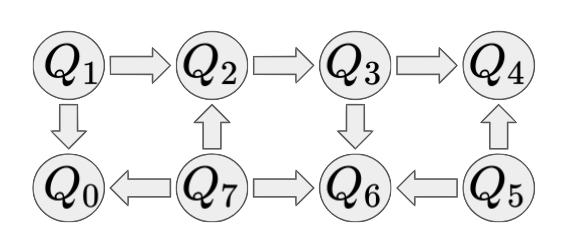
\includegraphics[width=5cm]{img/quantum-processor.png}
		\caption{The connectivity constraints of qubits on a quantum processor}
	\end{center}
\end{figure}
	
 
\subsubsection{Circuit Partitioning into Layers}

 First of all, the given quantum circuit is partitioned into several layers and a layer $l_i$ and all the quantum gates in a single layer $l_i$ do not share any qubits. Also, the number of the depth of a circuit is same as that of layers in the same circuit.
 
 After that, the qubit mapping is proposed in each layer $l_i$ and it does not have to correspond with that of the previous layer  $l_{i-1}$. Instead, a new layer of SWAP gates $\pi_i$ is inserted before the quantum compiler goes onto the next layer. In other words, the sequence of layers will be denoted as $l_0 \pi_1 l_1\pi_2 l_2 \dots$.
 
\subsubsection{Determining the Qubit Mapping}

The quantum compiler determines the mapping relationship between program qubits onto physical qubits on an actual quantum processor for each layer $l_i$, which is denoted as $\sigma^i_j: \{q_0, q_1, q_2, \dots q_{n-1}\} \rightarrow \{Q_0, Q_1, Q_2, \dots Q_{m-1}\}$. ($j$ is a unique id for that relationship, $n$ is the number of qubits on the given program, and $m$ is the number of physical qubits on a quantum processor) This relationship has to satisfy the CNOT-constraints on that hardware and the initial mapping is same of that of the previous layer, in other words, $\sigma^{i-1} = \sigma^i_0$.  The goal of this step is to find $\sigma^{i}$, which is the (sub-)optimal mapping relationship by adding minimum number of new operations by using an algorithm $A^{*}$ search.

\subsubsection{A* Search}
$A^{*}$ search is a state-space-based search algorithm that can be applied to states whose relationships have a tree structure.  The cost of the next node from the root to the node $x$ is $f(x)$, and $g(x)$ is the cost of the path from the root to the current state, and $h(x)$ is the additional cost of the link between the current state and the next state. 


Therefore, 
\begin{equation}
f(x) = g(x) + h(x)
\end{equation}

In the case of quantum compilation, the cost of the root state, which is the initial qubit mapping is 0. If the cost for the current state is $f(x)$, $g(x)$ is that of the previous mapping, and the $h(x)$ is the cost for additional layers.

If the current mapping $\sigma^i_j$ is followed by the next mapping  $\sigma^i_h$, the cost of the current mapping would be

\begin{equation}
 f(\sigma^i_j) = f(\sigma^i_j) + 7 \times \textrm{(number of SWAP gates)} 
\end{equation}
The equation above contains 7, because a single SWAP gate requires 7 elementary gates.

\begin{figure}[ht]
	\begin{center}
		\begin{tikzpicture}
			 \begin{yquant}
			qubit {$\ket0$} q[2];
	 		cnot q[1] | q[0];
			h q[0];
			h q[1];
			cnot q[1] | q[0];
			h q[0];
			h q[1];
			cnot q[1] | q[0];
			\end{yquant}
		\end{tikzpicture}
		\caption{7 elementary gates to implement a SWAP gate}
	\end{center}
\end{figure}

If you assign physical qubits $Q_c$ as a control qubit and $Q_t$ as a target qubit for a CNOT gate $g \in l_i$.  If the shortest directed path between $Q_c$ and $Q_t$ is denoted as $\hat{p}$, the additional gate cost for the CNOT gate $g$ in the current mapping $\sigma^i_j$ would be 

\begin{equation}
h(g, \sigma^i_j) = 7 \times (\hat{p} - 1)
\end{equation}

Therefore, the gate cost of additional layer $l$, which is $h(\sigma^i_j)$ is

\begin{equation}
h(\sigma^i_j) = max_{g \in l} h(g, \sigma^i_j)
\end{equation}

\subsubsection{Further Optimization}

In order to perform further optimization, the quantum compiler can incoroperate the information of not only the current layer, but also that of the next layer.  For example, the cost of the current layer can be

\begin{equation} 
h(\sigma^i_j) = max_{g \in l_i \cup l_{i+1}} h(g, \sigma^i_j)
\end{equation}

\newpage

\section{Distributed Computing}

 Distributed computing is the study of distributed system, which is a collection of several processors that are connected via network in order to solve a problem whose scale is much larger than what an individual processor can handle.  This type of computation involves message-passing between two physically separated processors to communicate and cooperate with each other by using pure HTTP, RPC, or message queues. \cite{distributedcomputingtext} 
 
 \subsection{Characteristics of Distributed System}
 \par Distributed system has the following characteristics, which are,
 
 \begin{itemize}
 
      \item No common physical clock 
      
      This is the key feature of distributed system because the clock of each processor runs at a different rate, so no clock can keep synchronized even after a single physical clock cycle.  Instead, distributed system depends on logical clock, which is common time platform for the whole system.
      
     \item No shared memory
     
     Each processor in a distributed system has its own memory space, rather than the common physical memory.  This feature indicates that a distributed system does not share its global state.
     
     
      \item Geographical separation
      
      The processors in a distributed system is located in different places, but they do not have to communicate with wide area network (WAN).  Actually, the network of workstations (NOW) and the cluster of workstations (COW) are becoming increasing popular because companies can easily purchase cost-efficient, high-speed, and ready-made processors. 
      
     \item Autonomy and heterogeneity
     
     A distributed system can work together even if it contains various processors which have different size, speed and operating system as long as they cooperate with one another.  This situation is regarded as "loosely-coupled".
     
\end{itemize}

\subsection{Advantages Over Computation by a Single Processor}

Performing computation in a distributed manner provides the following advantages.

\begin{itemize}
 
     \item{Computation by more than one entity}
     
     Applications such as money transfer (client-server) and reaching consensus among parties that are geographically separated (peer-to-peer) require information processing system that each processor can work together.
     
     \item{Resource sharing}
     
     Resource such as data in databases cannot be replicated because it is impossible or at least cost effective. Furthermore, allocating all the resource in just a single server is also not practical because the whole application would become unavailable if the server fails.  In order to solve these potential problems, the whole dataset is usually partitioned into several servers so that it can achieve more rapid access and higher reliability.
     
     \item{Access to geographically remote data and resources}
     
     Copying the whole dataset to every site is not desirable due to not only its predicted high cost, as I mentioned in the previous section, but also too sensitive.  Therefore, these large amount sensitive information, like user information collected by multinational cooperations are stored only in their central data centers and their oversea branches are only allowed to query them.
     
     \item{Enhanced reliability}
     
     Distributed system offers increased reliability due to its ability to replicate resource and achieve simultaneous execution of its given tasks. Also geographically distributed resources are highly unlikely crash or malfunction at the same time under normal circumstance.   This eliability entails several aspects.
     
     \begin{itemize}
     
      	\item{Availability}
	
	Resource become accessible at all times
	
      	\item{Integrity}
	
	The value and state of the resources should be always correct, especially users get concurrent access to those resources.	
	
      	\item{Fault-tolerance}
	
	Distributed system should be able to recover from its failure such as one of its server accidentally shutting down
	
    \end{itemize}
    
    
   \item{Increased performance / cost ratio}
   
     By resource sharing and access to geographically distant data, the performance and cost ratio of distributed system will improve more than using special parallel machines, this is particularly true of the NOW (network of workstation) setting.
     
\end{itemize}

\subsection{Task Allocation Problem}

Here are some definitions of the task allocation problem in distributed system. \cite{definition}
Given a distributed system $G = <V, E>$, where V is the set of nodes and E is the set of communication link between two different nodes, i.e. $\forall v_i. v_j \in V, \exists <v_i, v_j> \in E$.  The set of the resources in $a_i$ is $R_{a_i}$ and that required by the task $t$ is $R_t$.

\begin{enumerate}
	\item{$R_t \subseteq$ $\bigcup_{\forall a_i \in A_t} R_{a_i}$}
	\item{The objective should be either minimizing the execution time \cite{time} or maximizing reliability \cite{reliability}}
	\item{The nodes in $A_t$ can execute the allocated task under the constraint of the network structure $\forall a_i, a_j \in A_t \Rightarrow P_{ij} \subseteq E$ where $P_{ij}$ denotes the path between $a_i$ and $a_j$}
\end{enumerate}

Task allocation is known to be a NP-problem. \cite{np}

\subsection{Distributed Task Allocation Algorithms}

Due to the fact that task allocation problem is classified as NP-hard, many works have proposed heuristic functions for distributed task allocations in various settings.  Here, the author is going to introduce a simple objective function presented in the paper \cite{algorithm}, which is this work is based on.

It is assumed that a multicomputer system consists of $N$ heterogeneous processors with some amount of computational power and the size of memory.  Also, the given program includes $M$ communicating tasks, which is the nodes in the task interaction graph $G(V, E)$ ($V$ is $M$ communicating tasks and E is a set of communication relationship between two tasks).

The objective of this task allocation is to minimize the total execution time. In other words, the author has to come up with the optimal allocation $A$, which $A(i) = p$ indicates that the task $i$ is allocated to the processor $p$ and $TASKS_p$ is a group of tasks that are allocated to a processor $p$.

 The total execution in the heterogeneous computing cluster is same as the execution time in the most heavily loaded processor.  Two main types of costs should be considered.
 
 One is the execution cost.  The execution load in the processor $p$ is the cost of processing all the tasks that are assigned to $p$ for the allocation $A$. Suppose $C_{ip}$ is the cost of processing the task $i$ on the processor $p$, then the total execution cost on the processor $p$ is 
 
 \begin{equation}
 EXEC_p = \sum_{task \in  TASKS_p} C_{task, p}
 \end{equation}
 
  The other cost is the communication cost, which can be calculated by the following formula.

\begin{equation}  
COMM_p = \sum_{task \in TASKS_p} \sum_{(i=j), \\(i, j) \in E , \\ A(j) \neq p} d_{ij} * cc_{avg}
\end{equation}

 $d{ij}$ is the data sent between two communicating tasks between $i$, $j$ and $cc_{avg}$ is the average amount of transferring a data unit through the network transmission media.
  
 Therefore, the total cost for the processor $p$ is 
 \begin{equation}
 COST_p = EXEC_p + COMM_p
 \end{equation}
 Because the total execution time is equal to the execution of the most heavily loaded processor, the total execution time can be described as following.
 
 \begin{equation}
 COST =  max \{COST_p | 1 \leq p \leq n\}
  \end{equation}
 
 Therefore, the object function is $$min \,\,COST$$

\subsection{Models of Process Communication}

There are two basic models of process communication. One is \textit{synchronous} communication, which the sender process blocks its execution until it receives "acknowledgement " (or "ack" in short) from the receiver, which indicates that the receiver accepted the delivered message. In other words, the sender and receiver synchronize with each other, in order to adjust their timings to cooperate.
\par On the other hand, the other model, which is \textit{asynchronous} execution does not require synchronization between the sender and the receiver.  Therefore, the sender executes its following task right after it delivers its message to the receiver. 

\newpage

\section{Distributed Quantum Computing}
 
  Performing quantum computation on a cluster of middle-sized quantum processors is an easier approach compared to build a large single processor due to its lower physical requirement to build each processor \cite{distributedquantumcomputing}.  \\
This chapter explains several components that consists of distributed quantum computing system.

\subsection{Distributed Quantum Algorithms}

Distributed version of Shor's algorithm \cite{distributedshor} and Grover's algorithm \cite{distributedgrover}, both of which takes remote CNOTs (which will be discussed in a  later subsection) were presented in 2004 and 2012, respectively. 
However, the quantum circuits shown in these studies are physical ones, in other words, something that will be implemented directly on physical hardware, not something that users will implement in their programs. 

\subsection{Quantum Compiler for Distributed Quantum Computing}

 Quantum compiler is a software to optimize a quantum circuit defined in the given program to reduce the number of quantum gates and alleviate the effect of physical noise on that quantum state, and map that to the real hardware so that it will satisfy the connectivity constraint on that hardware \cite{qubitallocation}.  Just like the case of a local quantum software, distributed quantum computer also needs its distributed version in order to convert some CNOT gates into remote CNOTs and optimize both its execution time and the number of quantum gates in total, especially that of non-local operations.  This work focuses on the methodology to optimize the total execution time over the distributed quantum computing setting.
 
 \subsection{Gate-Teleportation-Based Non-Local CNOT}
 
Non-local operations are controlled operations between two qubits on two different processors there are three main approach to achieve them.

The first operation is the gate teleporation approach, and is also called non-local quantum gates \cite{gateteleportation} and telegate \cite{arithmetic}.  Here is the quantum circuit that achieve this operation.

Suppose that a person would like to apply a non-local CNOT between $|a_0\rangle$ on one processor and $|b_0\rangle$ on the other processor.  In order to do this, he has to prepare a new bell pair between these two processors.  ($|p_i\rangle$ in the following circuit diagram comes from p in $|\psi (psi)^+\rangle$)

 \begin{figure}[ht]
  	\begin{center}
  		\begin{tikzpicture}
   			\begin{yquant}
      				qubit {$\ket{\reg_{\idx}}$} a[1];
     				 qubit {$\ket{\reg_{\idx}}$} p[2];
     				 qubit {$\ket{\reg_{\idx}}$} b[1];
      				h p[0];
      				cnot p[1] | p[0];
      				cnot p[0] | a[0];
      				measure p[0];
      				x p[1] | p[0];
      				cnot b[0] | p[1];
      				h p[1];
      				measure p[1];
     				z a[0] | p[1];
   			\end{yquant}
		\end{tikzpicture}
		\caption{Quantum circuit for a non-local CNOT gate}
	\end{center}
\end{figure}

\newpage 

\subsection{Quantum Teleportation}

  Unlike classical communication, quantum states cannot be just copied and transmit to other nodes due to the no-cloning theorem, which forbids duplication of any quantum state.  However, a method called quantum teleportation \cite{teleportation} was proposed, which overcomes the restriction and allows sender to transmit single qubit state to a distant location. 
 		
This method requires both the single qubit state and a new Bell pair, and also the sender have to prepare two qubits and the receiver have to prepare one qubit.  After applying a CNOT gate and an H gate in the figure above, the sender have to measure both qubits and send those measurement results over the classical network.  After the receiver get those measurement results and apply some quantum gates if the measurement results of corresponding qubits on the sender's side are 1, in order to correct on the quantum state on the receiver's side.

\begin{figure}[ht]
  	\begin{center}
  		\begin{tikzpicture}
			\begin{yquant}
	 			qubit {$\ket{\reg_{\idx}}$} a[2];
	 			qubit {$\ket{\reg_{\idx}}$} b[1];	 
	 			h a[1];
	 			cnot b[0] | a[1];
	 			cnot a[1] | a[0];
	 			h a[0];
	 			measure a[0];
	 			z b[0] | a[0];
	 			measure a[1];
	 			x b[0] | a[1]; 	 
 			\end{yquant}
		\end{tikzpicture}
	\caption{Quantum circuit for quantum teleportation}
	\end{center}
\end{figure}

\subsection{Quantum-Teleportation-Based Non-Local CNOT}

 The second approach for performing a non-local CNOT gate is based on quantum teleportation mentioned in the previous section.  This approach assumes that every quantum processor has something called "communication qubits", which is a qubit that serves for communication purpose, unlike those used for computation purpose, which are called "data qubits".
 
 \begin{figure}[ht]
  	\begin{center}
  		\begin{tikzpicture}
			 \begin{yquant}
			 qubit {$\ket{\reg}$} control[1];
	 		 qubit {$\ket{\reg}$} comm1[1];
	 		 qubit {$\ket{\reg}$} comm2[1];
	 		 qubit {$\ket{\reg}$} control'[1];
	 		 qubit {$\ket{\reg}$} target[1]; 
	 
			 h comm1[0];
			 cnot comm2[0] | comm1[0];
	 		cnot comm1[0] | control[0];
	 		h control[0];
	 		measure control[0];
	 		z comm2[0] | control[0];
	 		discard control;
	 		init {$\ket{0}$} control;
	 		measure comm1[0];
	 		x comm2[0] | comm1[0];
	 		discard comm1;
			 init {$\ket{0}$} comm1;
			cnot control'[0] | comm2[0];
	 		cnot comm2[0] | control'[0];
			cnot control'[0] | comm2[0];
			box {$U$} target[0] | control'[0];
	 
 			\end{yquant}
			\end{tikzpicture}
			\vskip\baselineskip
			\begin{tikzpicture}
 			\begin{yquant}
			qubit {$\ket{\reg}$} control[1];
	 		qubit {$\ket{\reg}$} comm1[1];
	 		qubit {$\ket{\reg}$} comm2[1];
	 		qubit {$\ket{\reg}$} control'[1];
	 		qubit {$\ket{\reg}$} target[1]; 
	 
	 		cnot comm2[0] | control'[0];
	 		cnot control'[0] | comm2[0];
	 		cnot comm2[0] | control'[0];
	 
	 		h comm2[0];
	 		cnot comm1[0] | comm2[0];
	 		cnot comm2[0] | control'[0];
	 		h control'[0];
	 		measure control'[0];
	 		z comm1[0] | control'[0];
	 		discard control';
	 		init {$\ket{0}$} control';
	 		measure comm2[0];
	 		x comm1[0] | comm2[0];
	 		discard comm2;
	 		init {$\ket{0}$} comm2;
	 
	 		cnot control[0] | comm1[0];
			cnot comm1[0] | control[0];
			cnot control[0] | comm1[0];
	 
 			\end{yquant}
		\end{tikzpicture}

		\caption{The full quantum circuit for a teledata non-local controlled-U gate}
	\end{center}
\end{figure}
	
\newpage

\subsection{Data-Qubit-Swapping-Based Non-Local-CNOT}

The last approach for the non-local CNOT gate aims to sort qubits in the quantum processors so that each CNOT gates would be executed on the neighboring processors. (the paper \cite{distributedquantumcompiler} assumes linear topology)

\begin{figure}[ht]
  	\begin{center}
  		\begin{tikzpicture}
 			\begin{yquant}
 
			qubit {$\ket{\reg}$} Q_0[1];
			qubit {$\ket{\reg}$} Q_1[1];
			qubit {$\ket{\reg}$} Q_2[1];
			qubit {$\ket{\reg}$} Q_3[1];

			cnot Q_3[0] | Q_0[0];
			cnot Q_2[0] | Q_1[0];
			\end{yquant}
		\end{tikzpicture}

		\caption{The quantum circuit before the data qubit swapping occurs}
	\end{center}
\end{figure}
	
\begin{figure}[ht]
  	\begin{center}
  		\begin{tikzpicture}
			\begin{yquant}
 
			qubit {$\ket{\reg}$} Q_0[1];
			qubit {$\ket{\reg}$} Q_3[1];
			qubit {$\ket{\reg}$} Q_1[1];
			qubit {$\ket{\reg}$} Q_2[1];

			cnot Q_3[0] | Q_0[0];
			cnot Q_2[0] | Q_1[0];

 			 \end{yquant}
		\end{tikzpicture}
		\caption{The quantum circuit after the data qubit swapping occurs}
	\end{center}
\end{figure}	

\begin{algorithm}
 \caption{Algorithm for Data-Qubit Swapping}
 \begin{algorithmic}[1]
  \Require n-qubit circuit layer L with mod(n, 4) = 0 and $\frac{n}{2}$ CNOTs
  \Ensure  layer L with each CNOT operating on neighbor qubits
 \Function {Sort}{L}
    \If {$\exists \, CNOT(q_i, q_j)$ with $i, j \leq \frac{n}{2}$} 
   	\State{// $\exists \, CNOT(q_k, q_l)$ with $k, l > \frac{n}{2}$}
	\State{SWAP ($q_{i+1}$, $q_j$)}
	\State{SWAP($q_{k+1}$, $q_l$)}
	\State{L = L \textbackslash \{$q_i$,  $q_{i+1}$,  $q_{k}$,  $q_{k+1}$\}}
    \Else
	\State{// $\exists \, CNOT(q_{\frac{n}{2}}, q_l)$ with $l > \frac{n}{2}$}
	\State{// and $\exists \, CNOT(q_i, q_{l-1})$ with $i < \frac{n}{2}$}
	 \State{SWAP ($q_{\frac{n}{2}}$, $q_{l-1}$)}
	  \State{SWAP ($q_i$, $q_{\frac{n}{2}-1}$)}
	  \State{L = L \textbackslash \{$q_{\frac{n}{2}-1}$,  $q_{\frac{n}{2}}$,  $q_{l-1}$,  $q_{l}$\}}
    \EndIf
    
    \If {$L \neq \emptyset$}
    	\State{Sort(L)}
    \EndIf
    
\EndFunction

 \end{algorithmic} 
 \end{algorithm}

\newpage

 \subsection{Quantum Processor}
  A quantum processor, which corresponds to individual processor in a classical distributed system, has several qubits and links between two qubits in a limited topology.
  
  \begin{figure}[ht]
  	\begin{center}
  		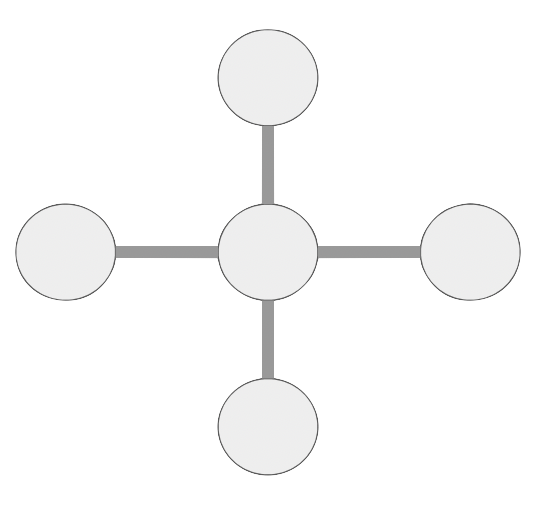
\includegraphics[width=5cm]{img/processor.png}
		\caption{An example of the layout of a quantum processor}
	\end{center}
\end{figure}
	
Usually, qubits in a current quantum processor are connected with a few neighboring qubits due to its physical restriction on a hardware.  Also, the error rate of a CNOT gate is much higher than that of a single quantum gate.
 
 \subsection{Communication Link for Distributed Quantum Computing}
Networking between two quantum processors need two types of communication links, which are classical links that transmit measurement results in the process of either telegate or teledata non-local CNOT gate, and quantum links that prepare create entanglement between the two qubits between the two neighboring quantum processors, or communication qubits of both processors.    

%\end{document}
%%% Local Variables:
%%% mode: japanese-latex
%%% TeX-master: "../thesis"
%%% End: